\subsection{Prototype}
Based on the data collected and analyzed from the survey described in the previous section, a prototype of a tool was designed and developed.
One of the main takeaways from the survey is that a majority of respondents felt a lack of awareness among their team members.
Based on that finding, the goal of the tool is to raise awareness about technical debt among the team members of a development team, about the strategy, decisions and priorities regarding technical debt in a project.
Further, the tool also aims to be a common source of information about the technical debt in a project and to be a helpful tool in discussions and decision making.

The prototype was developed as a web application with modern web technologies, React and Redux, using the programming language Typescript.
In order to speed up the development process, a component library, \textit{Material-UI}, was used to create the overall structure of the interface.
It consists of a main view with a dashboard containing multiple widgets containing information about the technical debt in the project.
The widgets are interconnected and responsive to user interaction.
In order to facilitate the evaluation, the prototype was developed with static data and no integration with live projects.
However, the prototype is coded with real data in mind, and could be integrated with source code repositories with more development.

Based on the work by Seaman and Guo \cite{seaman_measuring_2011}, review in the related work section, technical debt is represented in the prototype as "debt items" which are instances of debt that can be assigned to a location in the source code.
Each debt item includes, in addition to the location in the project, also a title, description, deadline, type and priority editable by the user.
The debt \textit{types} used in this study are informed by the \textit{dimensions od technical debt} defined by Tom et. al. \cite{tom_exploration_2013}.

\begin{figure}[h]
  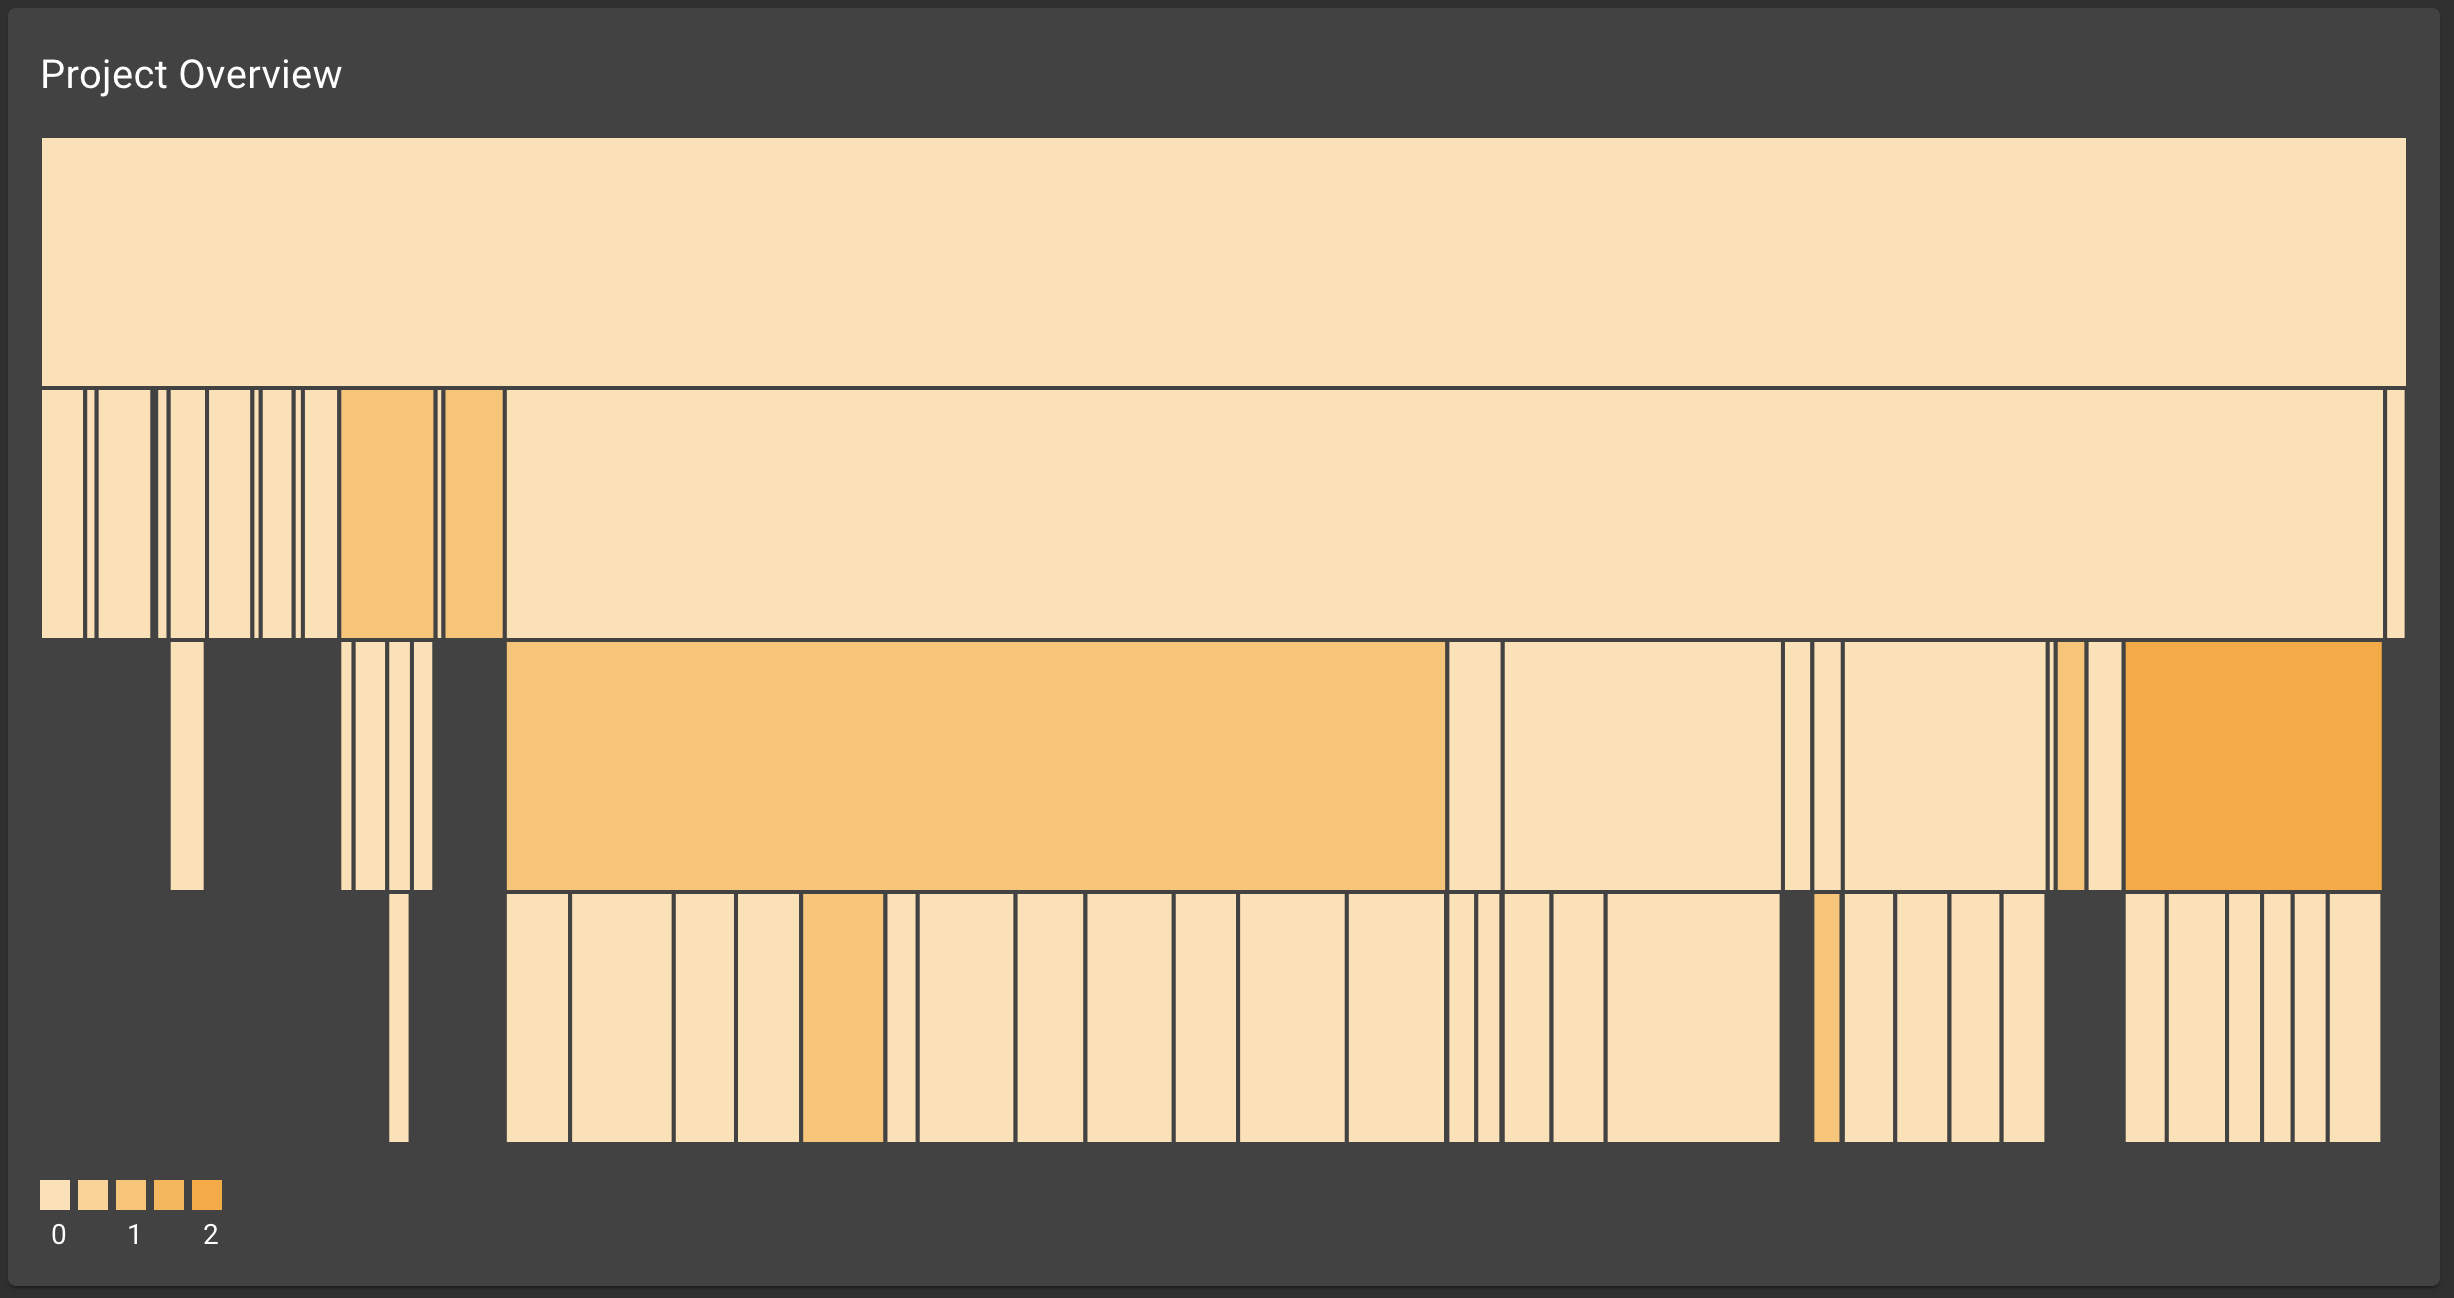
\includegraphics[width=\columnwidth]{overview}
  \Description{The overview visualization in the prototype.}
  \caption[Overview]{The overview visualization in the prototype.}
  \label{fig:overview}
  \centering
\end{figure}

The overview widget (figure \ref{fig:overview}) is a visualization of the source code hierarchical data.
Based on the work by Schultz et. al. reviewed in the related work section, two main visualization techniques were considered, \textit{treemaps} and \textit{icicle plots} \cite{schulz_design_2011}.
A \textit{treemap} would have the advantage of the overall size of the visual representation being decided by the size of the parent node, and thus easy to predict without knowing the size of the data set.
However it might decreases the perception of depth in the hierarchy and the parent nodes are often covered by its children nodes resulting in a less clear overview of the data.
Since the overview of the project is the main purpose of this visualization, the \textit{icicle plot} was decided to be a better choice since it uses adjacency to represent the relationship between nodes and gives all levels in the hierarchy the same amount of space and presents the whole data structure clearly.
It was also concluded by Woodburn et al. to be more intuitive and allow for easier navigation and understanding of the data \cite{woodburn_interactive_2019}.

Each file and folder in the tree structure is represented as a node, in this case a rectangle.
The layout is presented in a top down orientation implying that the top most node contains all nodes below it.
A node encodes three pieces of data, the location in the source code represented by the location in relation to other nodes, the size of the file or folder represented by the size of the node and the number of debt items associated with the node represented by the shade of the node.
The user can also interact with the visualization, more details are presented on demand when the user hovers over a node, and clicking on a node filters the backlog based on that location in the source code.

\begin{figure}[ht]
  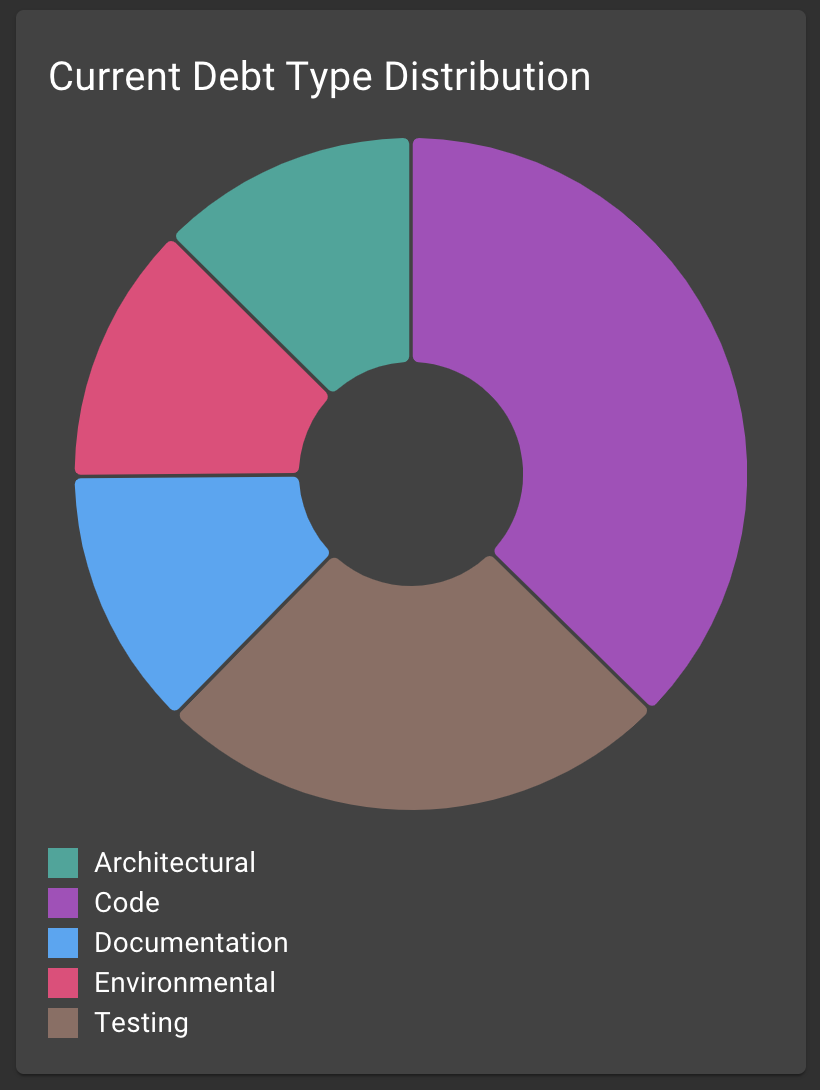
\includegraphics[width=\columnwidth]{debt-types}
  \Description{Prototype debt type visualization.}
  \caption[Debt types]{Prototype debt type visualization.}
  \label{fig:debt-type}
  \centering
\end{figure}

The debt type widget (figure \ref{fig:debt-type}) visualizes the distribution of debt types among the debt items in the project as a circle chart.
Each type corresponding to a distinct color which is recurring in other places in the prototype in order to help the user to find the type of a debt item at a glance.

\begin{figure}[h]
  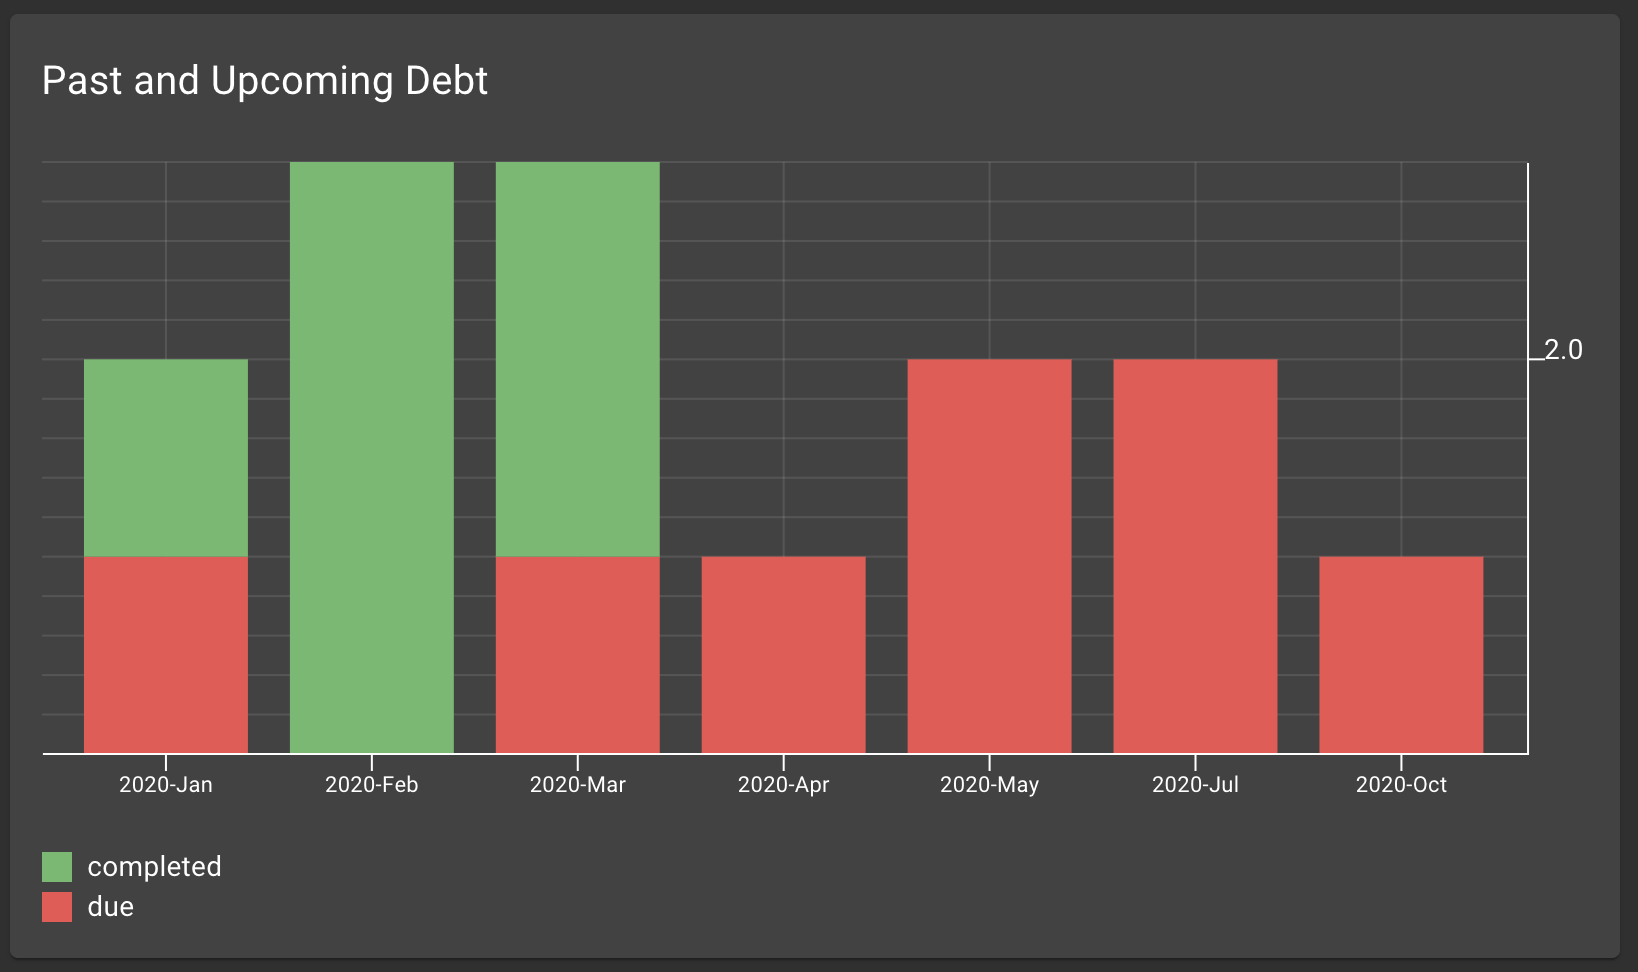
\includegraphics[width=\columnwidth]{history}
  \Description{The history visualization in the prototype.}
  \caption[Overview]{The history visualization in the prototype.}
  \label{fig:history}
  \centering
\end{figure}

To present the user with information about the evolution of debt in the project over a span of time, a timeline widget (figure \ref{fig:history}) is included in the prototype.
The timeline widget summarizes the number of debt items with deadlines for each month and visualizes this information as bar graph.
The bars include both completed (green) and non-completed (red) items colored by state.

\begin{figure}[h]
  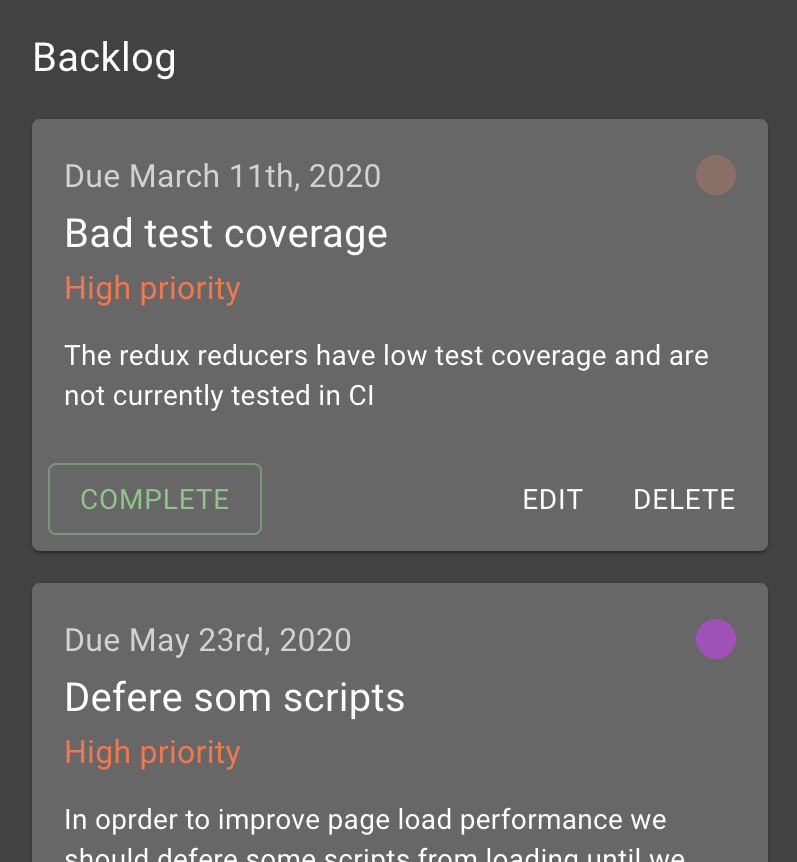
\includegraphics[width=\columnwidth]{backlog}
  \Description{The backlog column in the prototype.}
  \caption[Overview]{The backlog column in the prototype.}
  \label{fig:backlog}
  \centering
\end{figure}

The prototype also includes a column with cards (figure \ref{fig:backlog}) representing debt items, a "backlog" of items for the development team to work on. 
This is inspired by the approach proposed by Seaman and Guo where debt is presented as a "technical debt list" \cite{seaman_measuring_2011}.
The cards are sorted by priority and deadline with the highest priority debt items on top.
Each card presents all relevant information about a debt item and three action buttons: "complete", "edit" and "delete".
The user can also create a new debt item by clicking the button at the end of the list of cards.

The concept proposed in this study through this prototype aims to help development teams communicate about and manage technical debt by enabling everyone in the team to have an overview of the current technical debt status and priorities.
It allows the user to manage "debt items" representing an instance of debt somewhere in the project.
The user can create, edit and delete "debt items" which are presented as a backlog for the team to work on.
The user can also assign each item a deadline and priority. 
The goal is for this concept to be a common source of information about the teams strategy and priorities regarding technical debt, and also a help when making decision about technical debt in the project.
In other words, a unified interface for all kinds of debt in a project.